\chapter{Implementation of Data Converters}
\label{chapter:results}
\section{Sub-Circuits Used in Data Converters}

\subsection{Sample and Hold (S/H) Circuits}
Sample and hold (S/H) circuits or Amplifiers are required to sample the analog input signal and hold it during the full cycle of clock period give to the ADC.
\subsubsection{Basic S/H Topology}
\paragraph{Basic Configuration}
The basic sample-and-hold (S/H) circuit consists of an analog switch (typically implemented with a MOSFET) in series with a hold capacitor $C_H$. The input signal $V_{in}$ is sampled when the switch is closed, charging $C_H$ to $V_{in}$. When the switch opens, $C_H$ holds the sampled voltage, which can be read as $V_{out}$. The ON resistance $R_s$ of the switch and the value of $C_H$ determine the bandwidth and acquisition time of the circuit. The small-signal $-3$ dB bandwidth is given by:
\begin{equation}
    f_{-3\,\mathrm{dB}} = \frac{1}{2\pi R_s C_H}
\end{equation}
The acquisition time, i.e., the time required for $V_{out}$ to settle within a specified accuracy of $V_{in}$, is determined by the RC time constant. The basic configuration is shown in Figure~\ref{fig:basic_sh_config}.
\begin{figure}[h]
    \centering
    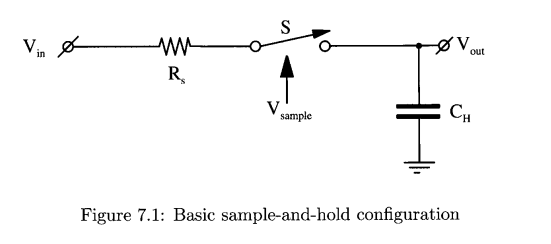
\includegraphics[width=0.5\textwidth]{figs/basic_sh_config.png}
    \caption{Basic Sample and Hold Circuit Configuration}
    \label{fig:basic_sh_config}
\end{figure}
by using a differential sample and hold circuit shown in Fig. \ref{fig}
the second order harmonic distortion can be avoided.
\begin{figure}
    \centering
    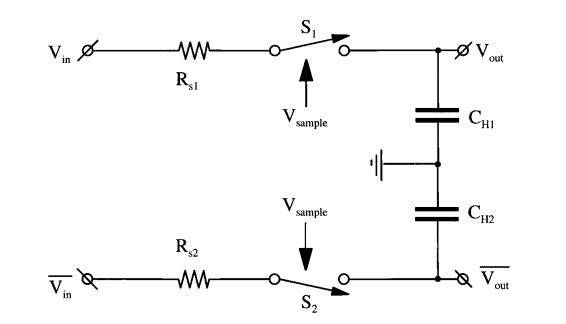
\includegraphics[width=0.7\textwidth]{figs/differential_sh.png}
    \caption{Differential Sample and Hold Circuit Configuration}
    \label{fig:differential_sh_config}
\end{figure}
\subsubsection{Integrated Sample and Hold Circuits}
Integrated sample-and-hold (S/H) circuits use operational amplifiers to improve accuracy, reduce charge injection, and provide buffering. A common topology is the integrating S/H circuit, as shown in Figure~\ref{fig:integrating_sh_circuit}. Here, the hold capacitor $C_H$ is connected between the output and the inverting input of an op-amp, forming an integrator. The analog switch $S$ samples the input signal onto $C_H$ when closed. When $S$ opens, the op-amp holds the voltage across $C_H$, providing a stable output.

\begin{figure}[h]
    \centering
    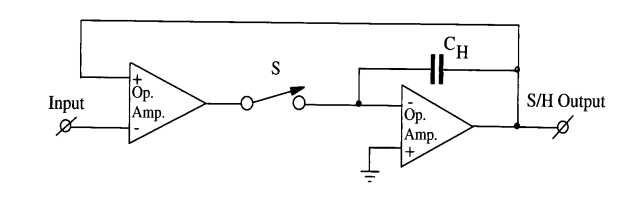
\includegraphics[width=0.7\textwidth]{figs/integrating_sh_config.png}
    \caption{Integrating sample-and-hold circuit}
    \label{fig:integrating_sh_circuit}
\end{figure}

This configuration minimizes the effects of charge injection and clock feedthrough by ensuring that the switch operates at a virtual ground. The op-amp buffer also isolates the hold capacitor from the load, improving hold accuracy. Special care must be taken in the design of the op-amp and switch to ensure low offset, high slew rate, and minimal leakage for precise sampling and holding.
\subsubsection{Practical integrated S/H circuit}
A practical example of an integrated sample-and-hold (S/H) circuit is shown in Figure~\ref{fig:practical_sh_circuit}. This circuit uses a differential input amplifier ($M_1$, $M_2$), loaded with a current mirror ($M_3$, $M_4$). The output current is integrated onto the hold capacitor $C_H$, which is connected between the drain and gate of the Miller stage transistor $M_6$. Biasing is provided by current source transistors $M_7$ and $M_8$, with their gates tied to a bias voltage $V_{bias}$. The sampling operation is controlled by switch $M_5$. During the track phase, $M_5$ is closed, allowing the output current to charge $C_H$ and track the input. When switched to hold mode, $M_5$ opens, and the voltage stored on $C_H$ is held, providing the output. This topology ensures low aperture uncertainty and minimizes the need for clock boosting circuits, as $M_5$ operates near the same gate-source voltage as $M_6$.

\begin{figure}[h]
    \centering
    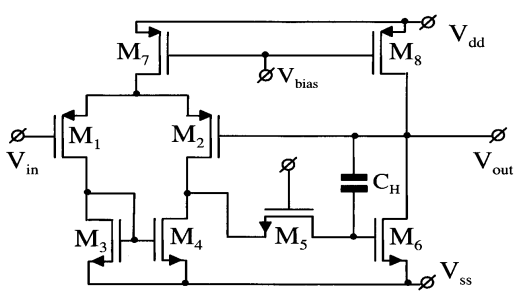
\includegraphics[width=0.7\textwidth]{figs/practical_sh_config.png}
    \caption{Integrated sample-and-hold circuit implementation}
    \label{fig:practical_sh_circuit}
\end{figure}

\subsection{Comparator Circuits}
Comparators are essential components in ADCs, used to compare the input signal with a reference voltage and produce a digital output indicating which is higher. They can be implemented using various techniques, each with its own advantages and trade-offs.
\begin{figure}
    \centering
    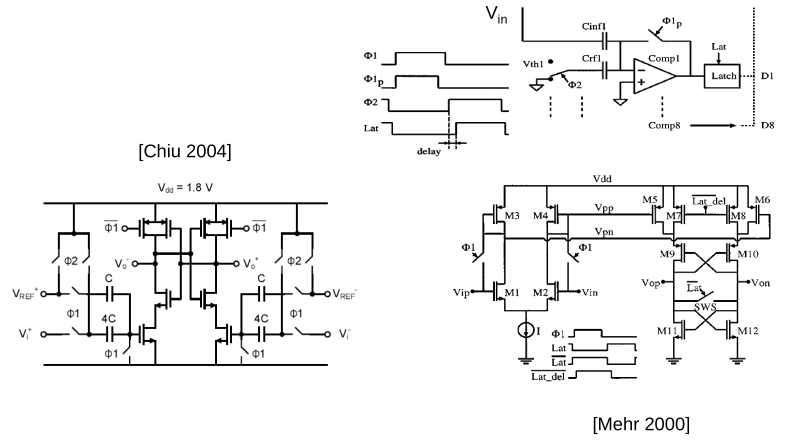
\includegraphics[width=0.7\textwidth]{figs/compartator_circuits.png}
    \caption{Few Comparator Circuits}
    \label{fig:comparator_circuit}
\end{figure}
\subsection{Digital-to-Analog Sub-Circuits}
\subsubsection{Binary-Weighted Current Source}
The binary-weighted current source DAC is a fundamental architecture that uses MOS transistors sized in binary ratios to generate output currents proportional to the digital input code. Each bit controls a current source whose value is weighted as a power of two, as shown in Figure~\ref{fig:binary_weighted_current_source}.

\begin{figure}[h]
    \centering
    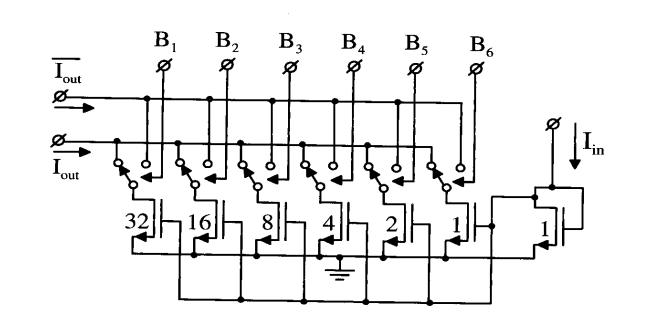
\includegraphics[width=0.8\textwidth]{figs/binary_weighted_current_source.png}
    \caption{MOS-only binary weighted current network}
    \label{fig:binary_weighted_current_source}
\end{figure}

In this structure, the reference current $I_{in}$ is mirrored and scaled by MOS transistors with widths proportional to $2^n$, where $n$ is the bit position. The output current $I_{out}$ is the sum of the selected currents, determined by the digital input bits $B_1$ to $B_N$:
\begin{equation}
    I_{out} = I_{ref} \sum_{k=0}^{N-1} b_k 2^k
\end{equation}
where $b_k$ is the $k$-th digital input bit.

\textbf{Advantages:}
\begin{itemize}
    \item Simple and fast operation.
    \item Direct current output, suitable for high-speed applications.
\end{itemize}

\textbf{Limitations:}
\begin{itemize}
    \item Requires precise current source matching and layout.
    \item Large area for high-resolution DACs due to exponential scaling of device sizes.
    \item Sensitive to channel length modulation and device mismatches.
\end{itemize}

\subsubsection{R-2R Ladder Network}
    The R-2R ladder network is a widely used architecture for implementing digital-to-analog converters (DACs) due to its simplicity, scalability, and ease of integration. It consists of resistors with only two values: $R$ and $2R$, arranged in a ladder-like structure. Each digital input bit controls a switch that connects the corresponding node either to a reference voltage or to ground, generating a binary-weighted output current or voltage.

    \begin{figure}[h]
        \centering
        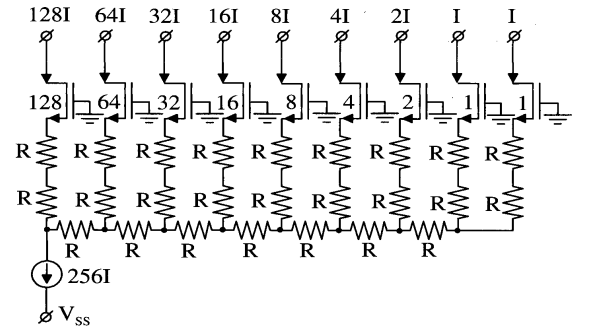
\includegraphics[width=0.85\textwidth]{figs/r2r_ladder.png}
        \caption{R-2R Ladder Network DAC Structure}
        \label{fig:r2r_ladder}
    \end{figure}

    The output voltage $V_{out}$ for an $N$-bit R-2R DAC can be expressed as:
    \begin{equation}
        V_{out} = V_{ref} \cdot \frac{1}{2^N} \sum_{k=0}^{N-1} b_k 2^{k}
    \end{equation}
    where $b_k$ is the $k$-th digital input bit (0 or 1), and $V_{ref}$ is the reference voltage.

    \textbf{Advantages:}
    \begin{itemize}
        \item Requires only two resistor values, simplifying layout and matching.
        \item Good linearity and monotonicity if resistor matching is precise.
        \item Easily scalable to higher resolutions.
    \end{itemize}

    \textbf{Design Considerations:}
    \begin{itemize}
        \item Resistor matching and layout are critical for accuracy.
        \item Output impedance and loading effects must be minimized.
        \item Parasitic capacitances can limit speed at high resolutions.
    \end{itemize}
    \subsubsection{MOS R-2R implementation}
    The MOS implementation of the R-2R ladder network replaces passive resistors with MOS transistors operating in the triode (linear) region, allowing for compact integration and process compatibility. Figure~\ref{fig:r2r_mos_elements} illustrates typical MOS-based R-2R cells and their possible configurations.

    \begin{figure}[h]
        \centering
        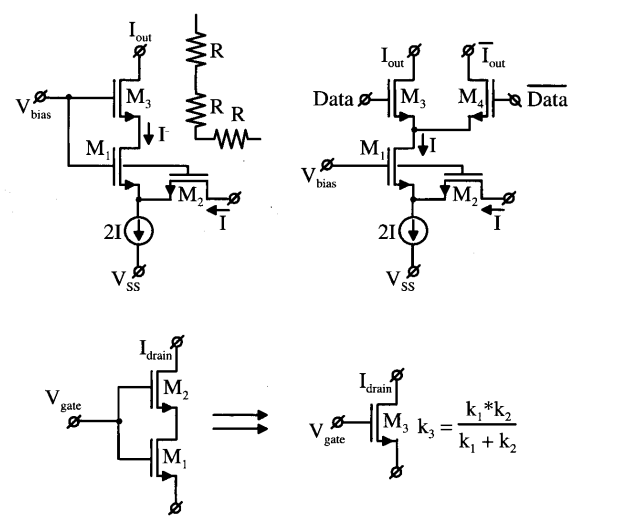
\includegraphics[width=0.85\textwidth]{figs/r2r_mos_elements.png}
        \caption{R-2R MOS elements: (a) Basic MOS R-2R cell, (b) Bit current switch integration, (c) Equivalent resistance using MOS transistors}
        \label{fig:r2r_mos_elements}
    \end{figure}

    In these circuits, matched MOSFETs ($M_1$, $M_2$, $M_3$, etc.) are biased such that their channel resistance emulates the required $R$ and $2R$ values. The current division and switching are achieved by controlling the gate voltages or digital data lines. When the MOSFETs operate in the triode region, their resistance is approximately:
    \begin{equation}
        R_{DS(on)} \approx \frac{1}{\mu_n C_{ox} \frac{W}{L} (V_{GS} - V_{th})}
    \end{equation}
    where $W/L$ is the transistor aspect ratio, $V_{GS}$ is the gate-source voltage, and $V_{th}$ is the threshold voltage.

    \textbf{Advantages:}
    \begin{itemize}
        \item Fully compatible with CMOS processes, enabling high integration.
        \item Area-efficient compared to passive resistor ladders.
        \item Programmable resistance by adjusting $W/L$ ratios or bias voltages.
    \end{itemize}

    \textbf{Limitations:}
    \begin{itemize}
        \item Non-idealities due to MOSFET mismatch, channel length modulation, and voltage dependence of $R_{DS(on)}$.
        \item Limited linearity and temperature stability compared to passive resistors.
        \item Careful biasing and layout are required for accurate operation.
    \end{itemize}

    This approach is especially useful in applications where integration density and process compatibility are prioritized over absolute accuracy.
\subsubsection{Capacitive DAC (CDAC)}
The capacitive digital-to-analog converter (CDAC) is a widely used architecture in CMOS technology due to its excellent matching properties, low power consumption, and ease of integration. The CDAC operates by redistributing charge among a binary-weighted array of capacitors, as shown in Fig. ~\ref{fig:binary_weighted_capacitor_dac}.

\begin{figure}[h]
    \centering
    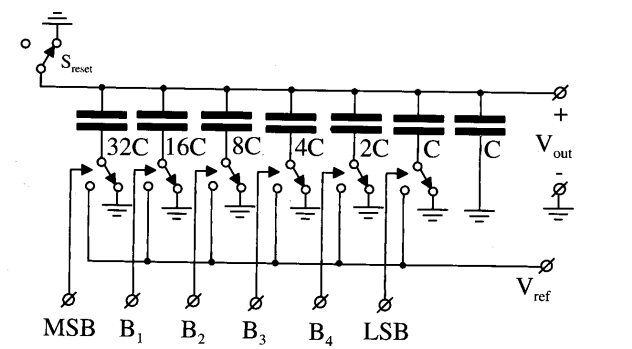
\includegraphics[width=0.85\textwidth]{figs/binary_weighted_capacitor_dac.png}
    \caption{Binary-weighted capacitor DAC structure}
    \label{fig:binary_weighted_capacitor_dac}
\end{figure}

\paragraph{Operation Principle}
The CDAC consists of $N$ binary-weighted capacitors ($C$, $2C$, $4C$, ..., $2^{N-1}C$) and a unit capacitor for charge balancing. Each capacitor can be switched between a reference voltage $V_{ref}$ and ground, depending on the digital input code. During operation, all capacitors are first discharged (reset phase). Then, based on the digital input, selected capacitors are connected to $V_{ref}$, while others remain at ground. The resulting output voltage is given by:
\begin{equation}
    V_{out} = \frac{V_{ref}}{2^N} \sum_{i=1}^{N} D_i \cdot 2^{i-1}
\end{equation}
where $D_i$ is the $i$-th digital input bit.

\paragraph{Advantages}
\begin{itemize}
    \item Excellent matching and linearity due to capacitor array.
    \item Low static power consumption.
    \item Fully compatible with CMOS processes.
\end{itemize}

\paragraph{Design Considerations}
\begin{itemize}
    \item Capacitor matching and layout symmetry are critical for accuracy.
    \item Parasitic capacitance and switch charge injection can affect performance.
    \item Output buffer is often required to prevent loading effects.
\end{itemize}

CDACs are commonly used in SAR ADCs and other mixed-signal systems where high linearity and integration are required.

% \subsection{Analog Multiplexers and Switches}
% \subsubsection{CMOS Transmission Gate}
% \subsubsection{Bootstrapped Switch}
% \subsubsection{On-resistance Variation and Signal Distortion}

% \subsection{Operational Amplifiers and Integrators}
% \subsubsection{Single-Stage and Two-Stage Op-Amps}
% \subsubsection{Miller Compensation}
% \subsubsection{OTA for Integrators in $\Sigma\Delta$ ADCs}
% OTAs are used in $\Sigma\Delta$ ADCs for integration and feedback.

% \subsection{Current Mirrors and Biasing Circuits}
% \subsubsection{Simple and Cascode Current Mirrors}
% \subsubsection{Bandgap Reference Circuits}
% \subsubsection{Biasing Techniques for Analog Blocks}

% \subsection{Timing and Control Logic (Brief Theoretical Overview)}
% \subsubsection{Clock Generation}
% \subsubsection{Control FSM for SAR Logic}
% \subsubsection{Latch Timing in Pipeline or Flash ADCs}

% \section{Summary}
% Interrelation of sub-circuits in ADC/DAC architectures.

% \section{Design Trade-offs}
% Speed vs power, accuracy vs area.
